\documentclass{article}
\usepackage{iclr2025_conference}

\usepackage[utf8]{inputenc}
\usepackage[T1]{fontenc}
\usepackage{lmodern}
\usepackage[colorlinks=true,linkcolor=black,citecolor=blue!60!black,urlcolor=blue!60!black]{hyperref}
\usepackage{url}
\usepackage{booktabs}
\usepackage{graphicx}
\usepackage{amsmath,amssymb}
\usepackage{subcaption}

% Numbers from outputs/final_metrics.json (regenerated by make_figures.py).
% \drawAttnNelboShort and \drawTTenNelbo are the epoch-30 value of the
% 60-epoch draw_attn_T10 run, stored in final_metrics.json under the key
% "draw_attn_T10_epoch30_test_nelbo" (105.54 -> rounded to 105.5).
\newcommand{\vaeNelbo}{102.9}
\newcommand{\vaeParams}{0.65M}
\newcommand{\vaeEpoch}{2.6}
\newcommand{\drawNoAttnNelbo}{93.8}
\newcommand{\drawNoAttnParams}{2.61M}
\newcommand{\drawNoAttnEpoch}{8.0}
\newcommand{\drawAttnNelbo}{99.7}            % at 60 epochs
\newcommand{\drawAttnNelboShort}{105.5}      % at 30 epochs (epoch-30 of 60-ep run)
\newcommand{\drawAttnParams}{0.87M}
\newcommand{\drawAttnEpoch}{14.0}
\newcommand{\drawTOneNelbo}{134.5}
\newcommand{\drawTFiveNelbo}{105.0}
\newcommand{\drawTTenNelbo}{105.5}            % T=10 at 30 epochs (same as above)

\title{Iterative generation with attention: \\ a study of DRAW against a vanilla VAE on MNIST}

\author{Oliver Wakeford, Ahzam Afaq, Said Abolhassan Razavi \\
M1 Artificial Intelligence and Data Science \\
Universit\'e Paris-Saclay}

\iclrfinalcopy

\begin{document}
\maketitle

\begin{abstract}
We compare a vanilla variational auto-encoder against the DRAW model of
\citet{gregor2015draw} on MNIST, with and without the Gaussian filterbank
attention. The single-shot VAE settles at a test negative ELBO of \vaeNelbo{}
nats per image after thirty epochs. Replacing it with a recurrent canvas of
\(T=10\) glimpses cuts that figure to \drawNoAttnNelbo{} nats at the same
budget. Adding attention reaches \drawAttnNelbo{} nats but only after sixty
epochs; under a matched thirty-epoch budget it actually trails the
no-attention variant at \drawAttnNelboShort{}. A short ablation on the number
of glimpses confirms that iteration is doing real work, going from
\drawTOneNelbo{} nats at \(T=1\) down to \drawTFiveNelbo{} at \(T=5\). The
samples line up with the numbers: DRAW produces noticeably sharper digits
than the VAE in either flavour. None of this is new on a dataset like MNIST,
but the comparison gives us a clean picture of where the recurrent and
attentional pieces of DRAW pay off, and where they cost more than they
return.
\end{abstract}

% ---------------------------------------------------------------
\section{Introduction}
\label{sec:intro}

Generative modelling of images sits at an awkward intersection. We want
models that capture rich structure, that we can sample from cheaply, and that
come with a tractable training objective. Variational auto-encoders
\citep{kingma2014vae,rezende2014stochastic} tick the last two boxes, and they
do so with a single forward pass through an encoder and a decoder. The price
is well known: VAE samples on natural-looking digits are usable but blurry,
and the latent space tends to collapse some directions if the architecture is
unbalanced.

DRAW \citep{gregor2015draw} attacks the blurriness from a different angle. It
keeps the variational training story but rebuilds the generator as a recurrent
network that writes onto a shared canvas across \(T\) timesteps. Each step
gets its own latent code, so the model can lay down a coarse sketch first and
then refine it. The paper goes one step further. Rather than reading or
writing the whole image at every step, a 2D Gaussian filterbank focusses
attention on a small patch, parameters and all learnt end-to-end.

We study three design dimensions in this report. Does the recurrent
canvas alone improve over the VAE on MNIST? Does the filterbank attention add
anything on top of iteration? And how sensitive is DRAW to the number of
glimpses? We trained the three configurations on the same dataset, with the
same optimiser and a matched thirty-epoch budget for the head-to-head, and
report the test ELBO bound, sample quality and the effect of \(T\). The
results are mostly what we expected, though the attention variant under a
limited training budget behaved differently enough to need a closer look.

% ---------------------------------------------------------------
\section{Related work}
\label{sec:related}

The variational auto-encoder reframed inference in deep latent variable models
as an optimisation problem over an amortised encoder, with the
reparameterisation trick making gradients tractable
\citep{kingma2014vae,rezende2014stochastic}. We use that framework throughout.

DRAW sits in the lineage of recurrent generative models. The motivating
observation is that humans do not draw a picture in one brushstroke, and
neither should a neural network if it is allowed to iterate. The recurrent
canvas idea predates DRAW in spirit, but DRAW combines it with the variational
encoder and with a soft, differentiable attention window built from two 1D
Gaussian filterbanks \citep{gregor2015draw}. The filterbanks are close in form
to the bilinear sampler later used in spatial transformer networks
\citep{jaderberg2015spatial}, although DRAW uses them on both the read and
the write side.

DRAW is not the only family that produces sharper images than vanilla VAEs.
Generative adversarial nets \citep{goodfellow2014gan} sidestep the
reconstruction objective entirely and end up with much crisper samples at the
cost of a harder training problem. Denoising diffusion models
\citep{ho2020ddpm} keep a likelihood-style objective but spend hundreds of
denoising steps at sample time. We do not run either of those here. They sit
on the menu as the obvious comparison points if compute were not a constraint.

The recurrent components of DRAW are LSTM cells \citep{hochreiter1997lstm},
and we trained both models with Adam \citep{kingma2015adam}.

% ---------------------------------------------------------------
\section{Method}
\label{sec:method}

\textbf{Vanilla VAE.} Given an image \(x \in [0,1]^{784}\), we model
\(p_\theta(x) = \int p_\theta(x|z)\, p(z)\, dz\) with \(p(z) = \mathcal{N}(0,I)\)
and a Bernoulli likelihood \(p_\theta(x|z) = \mathrm{Bern}(\sigma(f_\theta(z)))\).
An amortised encoder \(q_\phi(z|x) = \mathcal{N}(\mu_\phi(x), \mathrm{diag}\,
\sigma_\phi^2(x))\) gives the standard ELBO
\begin{equation}
\mathcal{L}(x;\theta,\phi) \;=\; \mathbb{E}_{q_\phi(z|x)}\!\left[\log p_\theta(x|z)\right]
\;-\; \mathrm{KL}\!\left(q_\phi(z|x) \,\|\, p(z)\right).
\label{eq:elbo}
\end{equation}
We train by minimising the negative of \eqref{eq:elbo}, summed over pixels.

\textbf{DRAW.} The generator becomes a recurrent network that maintains a
canvas \(c_t\) and a latent at every step. With encoder hidden state
\(h^{enc}_t\), decoder hidden state \(h^{dec}_t\) and the prior again standard
normal, the per-step recursion is
\begin{align}
\hat{x}_t &= \sigma(c_{t-1}), \quad x^{err}_t = x - \hat{x}_t \\
r_t &= \mathrm{read}(x, x^{err}_t, h^{dec}_{t-1}) \\
h^{enc}_t &= \mathrm{LSTM}^{enc}([r_t, h^{dec}_{t-1}], h^{enc}_{t-1}) \\
z_t &\sim q_\phi(z_t|h^{enc}_t) = \mathcal{N}(\mu_t, \sigma_t^2) \\
h^{dec}_t &= \mathrm{LSTM}^{dec}(z_t, h^{dec}_{t-1}) \\
c_t &= c_{t-1} + \mathrm{write}(h^{dec}_t).
\end{align}
The training loss is the BCE on \(\sigma(c_T)\) plus the sum of step KL terms,
which is the natural ELBO when the joint posterior factorises across
timesteps \citep{gregor2015draw}.

\textbf{Read and write.} The simple variant uses
\(\mathrm{read}(x,x^{err}) = [x, x^{err}]\) and a linear write that produces
a full \(28\times 28\) image. For attention, the decoder predicts five
parameters \((g_x, g_y, \log\sigma^2, \log\delta, \log\gamma)\) on each side;
these define an \(N\times N\) grid of Gaussian filters with centres
\((\mu^X_i, \mu^Y_j) = (g_x + (i - N/2 - 0.5)\delta,\, g_y + (j - N/2 - 0.5)\delta)\)
and shared variance \(\sigma^2\). The two 1D filterbanks
\(F_x \in \mathbb{R}^{N\times W}\), \(F_y \in \mathbb{R}^{N\times H}\) are
normalised per row, and the read becomes
\begin{equation}
\mathrm{read}_{attn}(x) \;=\; \gamma \cdot F_y\, x\, F_x^\top \in \mathbb{R}^{N\times N}.
\label{eq:read}
\end{equation}
The write places an \(N\times N\) patch back onto the canvas as
\(\gamma^{-1} F_y^\top \mathrm{patch}\, F_x\). We use \(N = 5\) throughout.

% ---------------------------------------------------------------
\section{Experimental setup}
\label{sec:setup}

\textbf{Data.} Standard MNIST \citep{lecun1998mnist}, 60{,}000 training images
and 10{,}000 test images, normalised to \([0,1]\). We treat pixel intensities
as Bernoulli probabilities so the BCE-with-logits loss matches the ELBO.

\textbf{Architectures.} The VAE has a 784\(\to\)400 ReLU encoder feeding two
20-dim heads, with a symmetric decoder. DRAW uses 256-unit LSTMs for both the
encoder and decoder, a 10-dim latent per timestep, and \(T=10\) steps for the
main runs. The attention variant uses an \(N=5\) read patch on both sides.
Parameter counts appear in Table~\ref{tab:results}. The no-attention DRAW is
actually the largest of the three, since its write head projects directly
into 784 pixels at every step. The attention variant only ever writes a
\(5\times 5\) patch, so it has a third of the parameters at the cost of
extra arithmetic to build the filterbanks.

\textbf{Training.} Adam \citep{kingma2015adam} with learning rate \(10^{-3}\),
batch size 128, and gradient clipping at norm \(5\). The VAE and the
no-attention DRAW each train for 30 epochs. We trained the attention variant
for 60 epochs and report both the epoch-30 value (matched-budget head-to-head)
and the final value (to give the filterbank parameters time to converge). The T-ablation
was 30 epochs throughout. We seed everything with 42, including PyTorch and
NumPy. All experiments ran on an Apple M5 Pro using the MPS backend.

\textbf{Evaluation.} We track the negative ELBO bound on the test set in nats
per image, summed over pixels. This is an upper bound on the negative
log-likelihood and the natural metric for this family of models.
Reconstructions come from passing a fixed test batch through the encoder and
decoder (or the full DRAW recurrence) and reading off \(\sigma(c_T)\).
Samples are drawn from the prior with no temperature trick.

\textbf{Reproducibility.} The code, the saved checkpoints and the
\verb|outputs/final_metrics.json| file from which the table values are pulled
are all in the project repository. Re-running \verb|train.py| and then
\verb|make_figures.py| regenerates every plot in this paper.

% ---------------------------------------------------------------
\section{Results}
\label{sec:results}

\begin{table}[t]
\centering
\small
\caption{Test negative ELBO on MNIST (lower is better), parameter counts and
mean training time per epoch on M5 Pro (MPS). The two DRAW-attn rows show
the matched-budget result (30 epochs) and the longer run (60 epochs).}
\label{tab:results}
\begin{tabular}{lcccc}
\toprule
Model & Params & Epochs & Test \(-\)ELBO (nats/img) & s/epoch \\
\midrule
VAE                              & \vaeParams        & 30 & \vaeNelbo            & \vaeEpoch \\
DRAW, no attention, \(T=10\)     & \drawNoAttnParams & 30 & \textbf{\drawNoAttnNelbo} & \drawNoAttnEpoch \\
DRAW, attention, \(T=10\)        & \drawAttnParams   & 30 & \drawAttnNelboShort  & \drawAttnEpoch \\
DRAW, attention, \(T=10\)        & \drawAttnParams   & 60 & \drawAttnNelbo       & \drawAttnEpoch \\
\bottomrule
\end{tabular}
\end{table}

\begin{figure}[t]
\centering
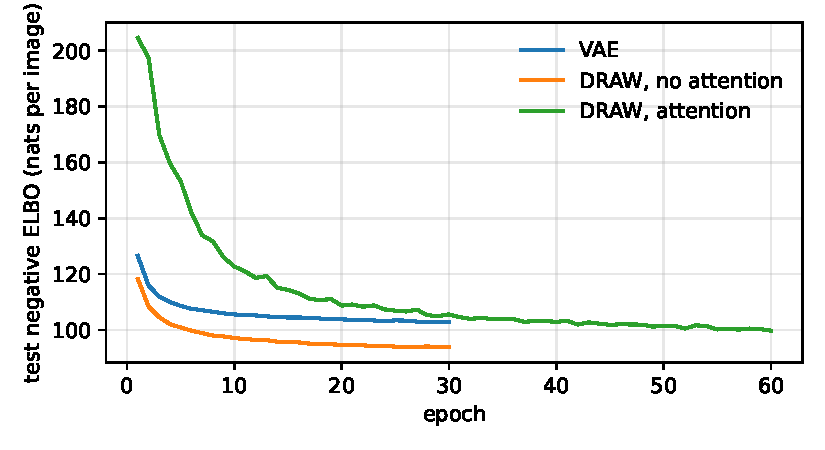
\includegraphics[width=0.85\linewidth]{figures/training_curves.pdf}
\caption{Test negative ELBO (nats per image) across training epochs. The
no-attention DRAW pulls ahead of both the VAE and its attention sibling
within ten epochs. Attention closes some of the gap given more training but
does not catch up here.}
\label{fig:curves}
\end{figure}

The headline numbers are in Table~\ref{tab:results} and Figure~\ref{fig:curves}.
The vanilla VAE plateaus around \vaeNelbo{} nats roughly halfway through
training and barely moves after that. DRAW without attention drops below it
within five epochs and ends at \drawNoAttnNelbo{} nats, which is roughly what
we expected from an iterative model on a simple dataset.

The twist is the attention variant. At a matched 30-epoch budget it lands at
\drawAttnNelboShort{} nats, slightly worse than the VAE and well behind the
no-attention DRAW. Letting it run for another 30 epochs brings it down to
\drawAttnNelbo{}, which beats the VAE but still trails no-attention DRAW.
We think the bottleneck is capacity. The no-attention write head has a
direct \(256 \to 784\) projection at every step, so a single linear write is
already expressive enough to redraw most of the canvas. The attention write
only ever puts down a \(5\times 5\) patch, which has to be carefully placed
to be useful. That is more parameter-efficient (\drawAttnParams{} versus
\drawNoAttnParams{}) but it makes optimisation harder, especially on a
small image where the no-attention model is not really compute-limited.

\begin{figure}[t]
\centering
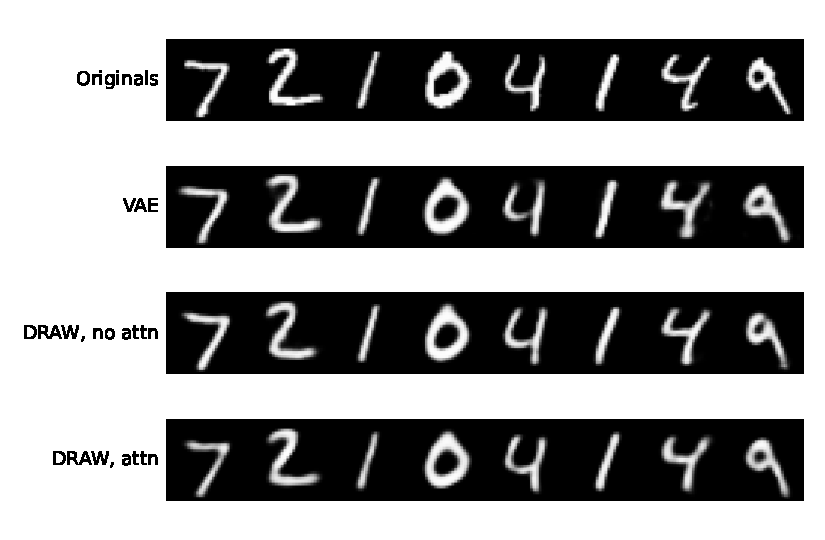
\includegraphics[width=0.95\linewidth]{figures/reconstructions.pdf}
\caption{Reconstructions of a fixed test batch. Top: originals. The two DRAW
rows reconstruct strokes more sharply than the VAE, which smears thin lines
and round digits like 3 and 8.}
\label{fig:recon}
\end{figure}

\begin{figure}[t]
\centering
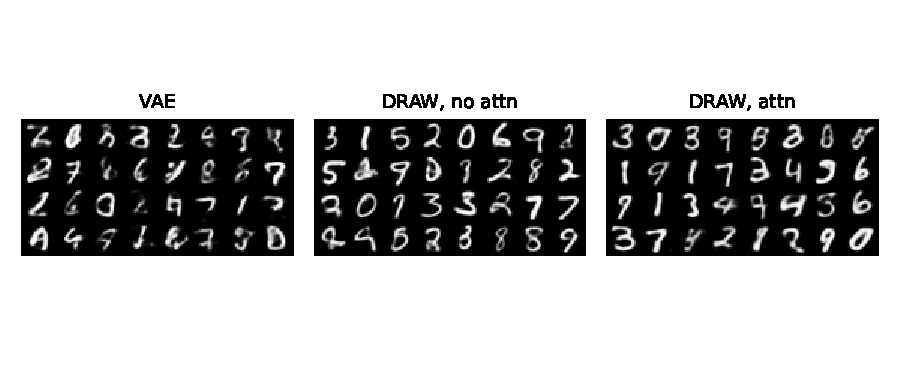
\includegraphics[width=0.95\linewidth]{figures/samples.pdf}
\caption{Random samples from the prior. The VAE produces blurry digit-like
shapes; both DRAW variants give sharper outlines, with attention adding the
most visible cleanup of stroke endings and the occasional broken digit when
the attention window misses the centre.}
\label{fig:samples}
\end{figure}

The reconstructions in Figure~\ref{fig:recon} tell a similar story. The VAE
captures the overall shape but smears thin strokes, while both DRAW rows
reproduce digits with cleaner edges. The qualitative gap is more obvious in
the random samples (Figure~\ref{fig:samples}). Visually, attention does pay
off here even where the ELBO disagrees, with crisper stroke endings on most
samples. It also produces the occasional malformed digit, which we put down
to the attention window drifting off the canvas centre. This tends to happen with DRAW on small images, and longer training or a
larger \(N\) should reduce it.

\begin{figure}[t]
\centering
\begin{minipage}[t]{0.49\linewidth}
  \centering
  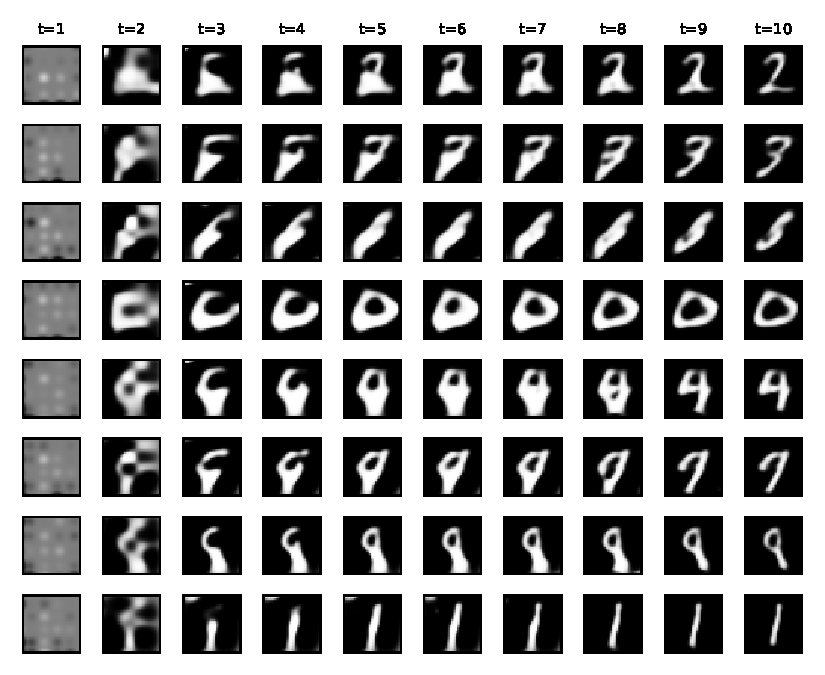
\includegraphics[width=\linewidth]{figures/draw_steps.pdf}
  \caption{Eight DRAW samples shown after each of the \(T=10\) attention
  glimpses. The model starts with a vague blob and tightens it over
  successive writes.}
  \label{fig:steps}
\end{minipage}\hfill
\begin{minipage}[t]{0.49\linewidth}
  \centering
  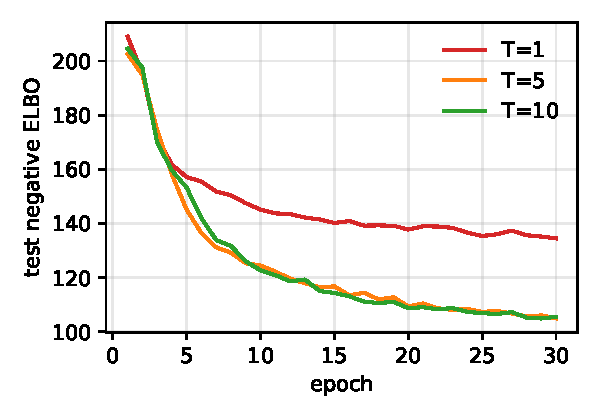
\includegraphics[width=\linewidth]{figures/t_ablation.pdf}
  \caption{Ablation on the number of glimpses for DRAW with attention.
  \(T=1\) is essentially a one-step recurrent VAE; gains from extra
  iterations saturate by \(T=5\) at this training budget.}
  \label{fig:tabl}
\end{minipage}
\end{figure}

The step-by-step samples in Figure~\ref{fig:steps} make the iterative story
visible. After one or two glimpses the canvas barely encodes a digit; by the
sixth or seventh the rough outline is in place and the rest of the steps
sharpen it. The ablation in Figure~\ref{fig:tabl} confirms that this is doing
real work. With \(T=1\) the model behaves like a one-shot VAE with extra
parameters and lands at \drawTOneNelbo{} nats, by far the worst of the
ablation. \(T=5\) drops it to \drawTFiveNelbo{}, and \(T=10\) at the same
budget gives \drawTTenNelbo{}. The marginal gain from going past \(T=5\) is
essentially zero at 30 epochs and only opens up with longer training. This is consistent with the original paper's finding that a
handful of steps captures most of the gain.

Regarding training cost: the attention variant is roughly five times slower per
epoch than the VAE and twice as slow as no-attention DRAW, due to the
per-timestep filterbank construction. For MNIST that is a fair price, but
the cost would scale poorly to higher resolutions where the filterbank
matrices grow with the image size.

% ---------------------------------------------------------------
\section{Conclusion}
\label{sec:conclusion}

DRAW beats a vanilla VAE on MNIST in both ELBO and sample quality, and
iteration is doing real work as the T-ablation shows. The surprise was that
the attention variant did not improve over no-attention DRAW under a
matched training budget on this small dataset, although it does pull closer
with twice the epochs. Put plainly, a \(28\times 28\) canvas with a
256-unit write head is not really capacity-limited, so the
parameter-efficient attention pays for itself slowly.

\textbf{Limitations.}
Several choices constrain what we can conclude. All results come from a
single random seed, so we have no variance estimate on the ELBO numbers.
The head-to-head comparison uses only thirty epochs, which is enough for
the VAE and no-attention DRAW to converge but not for the attention
variant, making the comparison somewhat unfair. We did no hyperparameter
search: the learning rate, hidden size, latent dimension and patch size
\(N\) were all fixed at the values from the original paper or at round
numbers that fit comfortably in laptop memory. The latent dimension for
DRAW (\(z=10\) per step) is small enough that the model may be
underpowered relative to what the paper reports. Finally, we use soft
pixel values in \([0,1]\) rather than binarising the inputs, which means
our ELBO numbers are not directly comparable to those in the original
paper.

\textbf{Possible improvements.}
The most straightforward extension is to switch to properly binarised
MNIST and train for at least a hundred epochs, which is the regime the
original paper evaluates in and where we would expect attention to show a
cleaner advantage. Increasing the patch size from \(N=5\) to \(N=12\)
would give the attention write head more expressive power per step.
A KL-annealing schedule, where the weight on the KL term is ramped up
from zero over the first few epochs, is a common stabilisation trick for
DRAW that we did not use and that would likely help the attention variant
converge faster. Finally, testing on a harder dataset such as SVHN or
Omniglot would give a clearer picture of whether the filterbank attention
is worth its training cost outside the toy regime.

\bibliography{references}
\bibliographystyle{iclr2025_conference}

\end{document}
